\section{Turing Maschine}
\label{turingmaschine}
Die Turingmaschine wurde 1936 von Alan Turing entwickelt und ist rein theoretisch, denn eine Maschine exakt wie es Turing beschreibt wurde niemals gebaut, da dies auch nicht sinnvoll wäre. Turing entwickelte diese Theorie aufgrund des Entscheidungsproblem von David Hilber und Wilhelm Ackermann \cite{theessentialturing}. Die Turing Maschine ist die heutige Grundlage vieler Programmiersprachen, wie Java, C++ oder Phyton. Diese Programmiersprachen werden auch als Turing complete bezeichnet, was so viel heißt wie dass die Turing Maschine diese theoretischer weiße emulieren kann.

\subsection{Funktion} 
Die Turing Maschine beinhaltet lediglich zwei Bauteile.
\begin{enumerate}
\item  Ein unendlich langes Band, dass in eine Kette von horizontalen Kästchen eingteilt ist. Jedes dieser Kästchen kann entweder eine 0,eine 1 oder auch nichts beinhalten. Zudem kann das Band nach rechts und nach links verschoben werden.
\item Ein Kasten auch "Heap" oder auch "Scanner" genannt, der die Zahlen auf dem Band einlesen, löschen und ändern kann.
\end{enumerate}
 
\begin{figure}[hbtp]
\centering
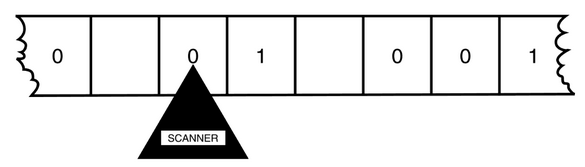
\includegraphics[scale=1]{TuringmashinePicture.png}
\caption{Beispielhafte Darstellung einer Turing Maschine\cite{theessentialturing}}
\end{figure}

\subsection{Beispiel} Zur besseren Vorstellung, erkläre ich das Ganze nochmal an einem Beispiel. Nehmen wir mal an wir wollen, dass die Turing Maschine für uns unendlich Hochzählt. So kann man dies mit nur zwei einfachen Befehlen ausführen. 

\begin{itemize}
\item Befehl 1 = Bei einer 1, ändere diese in eine 0 und gehe nach links 
\item Befehl 2 = Bei einer 0 oder einer Lücke, ändere diese in eine 1 und gehe zum letzten Bit der Zahl 
\end{itemize}

Die Befehle für die Turing Maschine kann man sich also heute wie die Programme auf unseren Computern vorstellen.

\subsection{Codebeispiel}
Dieser Code aus Java macht praktisch genau das Selbe, wie das kleine Beispielprogramm der Turing Maschine. Das Einzige was auffällt ist, dass dieses Programm nur bis 1000 zählt, da unsere Turing Maschine einen unendlichen Speicher besitzt anders wie jeder PC auf der Welt.

\begin{minted}{java}
for (int i = 0; i < 1000; i++) {}			
\end{minted}